\chapter{Thermal Expansion}
\label{ch:thermalExpansion}

\section{Necessity of Modeling}
  % discuss the EBR-II tests
  % TODO discuss that it is assumed user input is at ``cold'' conditions
  Steel props from \cite{ht9Prop}.
  Fuel props from \cite{thexpU10Zr}.

  \begin{figure}
    \centering
    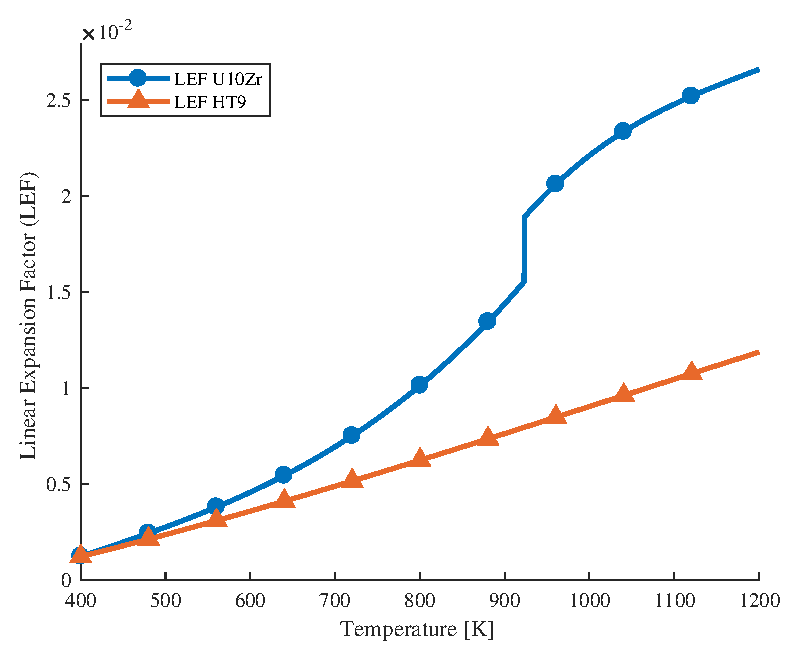
\includegraphics[width=0.7\textwidth]{lef_plot}
    \caption{Linear Expansion Factor for HT9 Steel and U10Zr Fuel.}
    \label{fig:lef_plot}
  \end{figure}

\section{Model Details}
  Highly detailed thermal expansion modeling can be done using the Finite
  Element Method to calculate local stresses and strains on all reactor
  structural components. However, the model developed here for the simulation of
  SFRs does not estimate temperature and heat generation at all positions due to
  the smearing of hexagonal assemblies. Therefore, a simplified thermal
  expansion model is developed to simulate the effect of thermal expansion on
  reactivity.

  In the model, linear dimensions are expanded based on material properties.
  All sodium in the reactor is assumed to be liquid so effects of thermal
  expansion within the sodium are assumed to be described by the change in
  density as a function of temperature as described by state equations in
  \cite{sodiumProp}. Additionally, the mass of sodium within the reactor is not
  conserved. Sodium in the coolant is allowed to flow into and out of an
  expansion vessel external to the reactor. In a SFR, sodium in the bond region
  flows upward from the fuel region into a gas plenum; however, this is not
  modeled as the sodium level in the bond is not tracked. Instead, the mass of
  sodium in the bond region is allowed to vary during the simulation.

  All structural materials in the reactor are modeled as HT9 stainless steel.
  Fuel material is modeled as metallic uranium with 10\% Zr by weight included
  (i.e. U10Zr). Thermal expansion properties for HT9 are given in \cite{ht9Prop}
  and for U10Zr are given in \cite{thexpU10Zr}. The equations for the Linear
  Expansion Factor (LEF) as functions of temperature as used in this application 
  are given
  \begin{equation}
    \label{eq:lef_ht9}
    \left( \frac{\Delta L}{L} \right)_{\text{HT9}} = 
      -2.191 \times 10^{-3} + 5.678 \times 10^{-6} \, T + 
      8.111 \times 10^{-9} \, T^2 - 2.576 \times 10^{-12} \, T^3 
  \end{equation}
  \begin{multline}
    \label{eq:lef_u10zr}
    \left( \frac{\Delta L}{L} \right)_{\text{U10Zr}} = \\
      \begin{cases}
        -7.3 \times 10^{-3} + 3.489 \times 10^{-5} \, T 
          - 5.154 \times 10^{-8} \, T^2 + 4.39 \times 10^{-11} \, T^3 & 
          T \le 923 \units{K} \\
        -0.25252 + 6.669 \times 10^{-4} \, T - 5.441 \times 10^{-7} \, T^2 
          + 1.518 \times 10^{-10} \, T^3 & \text{otherwise}
      \end{cases}
  \end{multline}
  for $T$ in \units{K}. Note that U10Zr has a phase change at 923 \units{K} that 
  increases the LEF at this point. The LEF of HT9 and U10Zr over the range of
  operating temperatures of SFRs are plotted in \fref{fig:lef_plot}.  It is 
  observed that the LEF of U10Zr is as much as twice that of HT9. This implies
  fuel material will expand significantly more than structural material which is
  expected behavior for metallic fuel.

  To simplify the modeling of thermal expansion, material dimensions are
  uniformly expanded in radial and axial directions. It is assumed that material
  expansion in the radial direction (both $x$ and $y$ directions) expands
  as HT9 because the dominating expansion in this direction is
  due to the expansion of the hexagonal assemblies themselves. It is assumed 
  that material expansion in the axial direction (the $z$ direction) expands
  as U10Zr because the dominating expansion in this direction is the elongation
  of the metallic fuel. Within a hexagonal assembly, all dimensions are expanded
  as HT9 with the exception of the fuel radius, $R_F$, which is expanded as 
  U10Zr. Within a hexagonal assembly, the coolant flow area and the sodium bond
  area are allowed to ``float'' because they are assumed liquid. All dimensions
  in the reactor are expanded assuming the user-input dimensions are at
  room-temperature conditions and using a single, fixed thermal expansion
  temperature $T_{exp}$. The expansion temperature should be selected to
  represent the average temperature within the reactor. It is expected thermal
  expansion effects will be significant. However, thermal expansion factors are
  typically on the order $10^{-6}$ so small, local changes in temperature are
  will not affect the macroscopic simulation.

  Given the assumptions of this model, a radial thermal expansion factor can be
  defined using \eref{eq:lef_ht9} as
  \begin{equation}
    \label{eq:lef_r}
    F_r(T_{exp}) = \left(\frac{\Delta L}{L}\right)_{\text{HT9}}
  \end{equation}
  which is a function of $T_{exp}$. Note that given the assumption of uniform
  radial thermal expansion, ${F_x(T_{exp}) = F_y(T_{exp}) = F_r(T_{exp})}$.
  Similarly, an axial thermal expansion factor can be defined using
  \eref{eq:lef_u10zr} as 
  \begin{equation}
    \label{eq:lef_a}
    F_a(T_{exp}) = \left(\frac{\Delta L}{L}\right)_{\text{U10Zr}}
  \end{equation}
  and $F_a(T_{exp}) = F_z(T_{exp})$.

  % define volume expansion factor
  % prove areas do not expand if all at same rate

\section{Implementation}
  Thermal expansion effects the reactor simulation in two major ways. First,
  thermal expansion causes the physical dimensions of the reactor to increase. 
  This is modeled by the expansion of individual elements in the solution of the
  finite element method as well as the expansion of areas within the hexagons.
  Second, as a result in the increase in physical dimensions, the density of
  reactor materials decreases. This decrease in density is necessary to preserve
  the mass of the materials within the reactor. The density change is observed
  as an effect on cross-sections.

  The conservation of reactor material is expressed as a conservation of number
  of atoms. Allow the superscript $H$ to represent ``Hot'' conditions (i.e.
  thermally expanded) and the superscript $C$ to represent ``Cold'' conditions.
  Then, the conservation of the number of atoms for species $i$, can be
  expressed as
  \begin{equation}
    \label{eq:conservation}
    n_i^H = n_i^C 
  \end{equation}
  where $n_i^H$ is the number of atoms of species $i$ after thermal expansion.
  The number of atoms $n_i$ can be written as 
  \begin{equation}
    \label{eq:nden_definition}
    n_i = N_i \, V_i
  \end{equation}
  where $N_i$ is the number densities of species $i$ and $V_i$ is the volume
  occupied by species $i$. Then, inserting \eref{eq:nden_definition} into 
  \eref{eq:conservation} yields an expression for the thermally expanded number
  density of species $i$ as
  \begin{align}
    N_i^H \, V_i^H &= N_i^C \, V_i^C, \\
    N_i^H &= N_i^C \frac{V_i^C}{V_i^H}
  \end{align}
  where the term $\frac{V_i^C}{V_i^H} < 1$ and represents the expansion of the
  volume occupied by species $i$.

  \subsection{Expansion of Elements and Area Fractions}
    

  \subsection{Cross-section Effects}

\section{Results}
  \begin{figure}
    \centering
    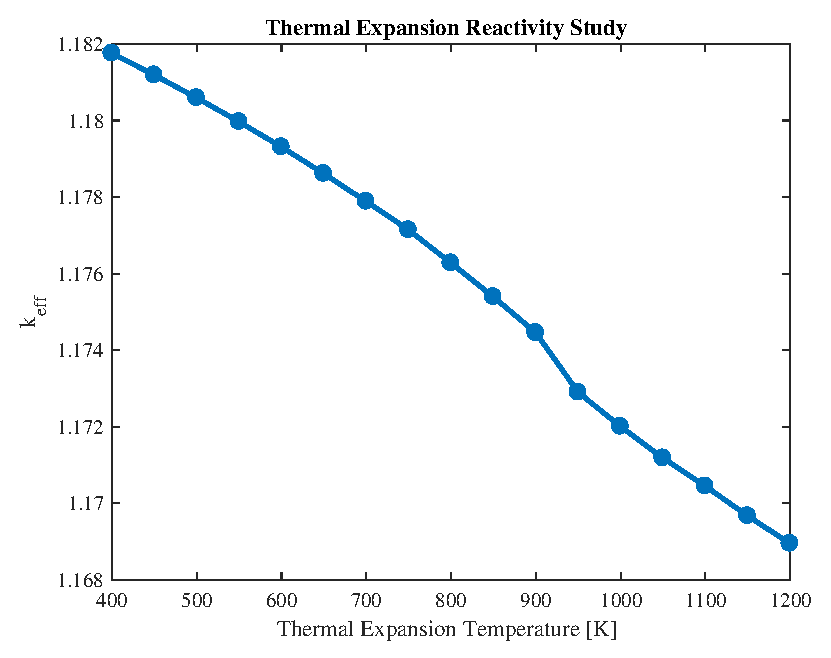
\includegraphics[width=0.7\textwidth]{thexp_study}
    \caption{Reactivity due to Thermal Expansion Temperature.}
    \label{fig:thexp_study}
  \end{figure}

